\chapter{Description du sujet}

\section{Qu'est-ce que SecuCom ?}

\textbf{SecuCom} est une plateforme de gestion sécurisée spécifiquement conçue pour les secrétariats sociaux et leurs entreprises clientes. Elle se présente sous la forme d'une application web offrant des espaces privés distincts où les différents acteurs peuvent interagir et gérer leurs données administratives de manière fluide et sécurisée.

\begin{figure}[H]
    \centering
    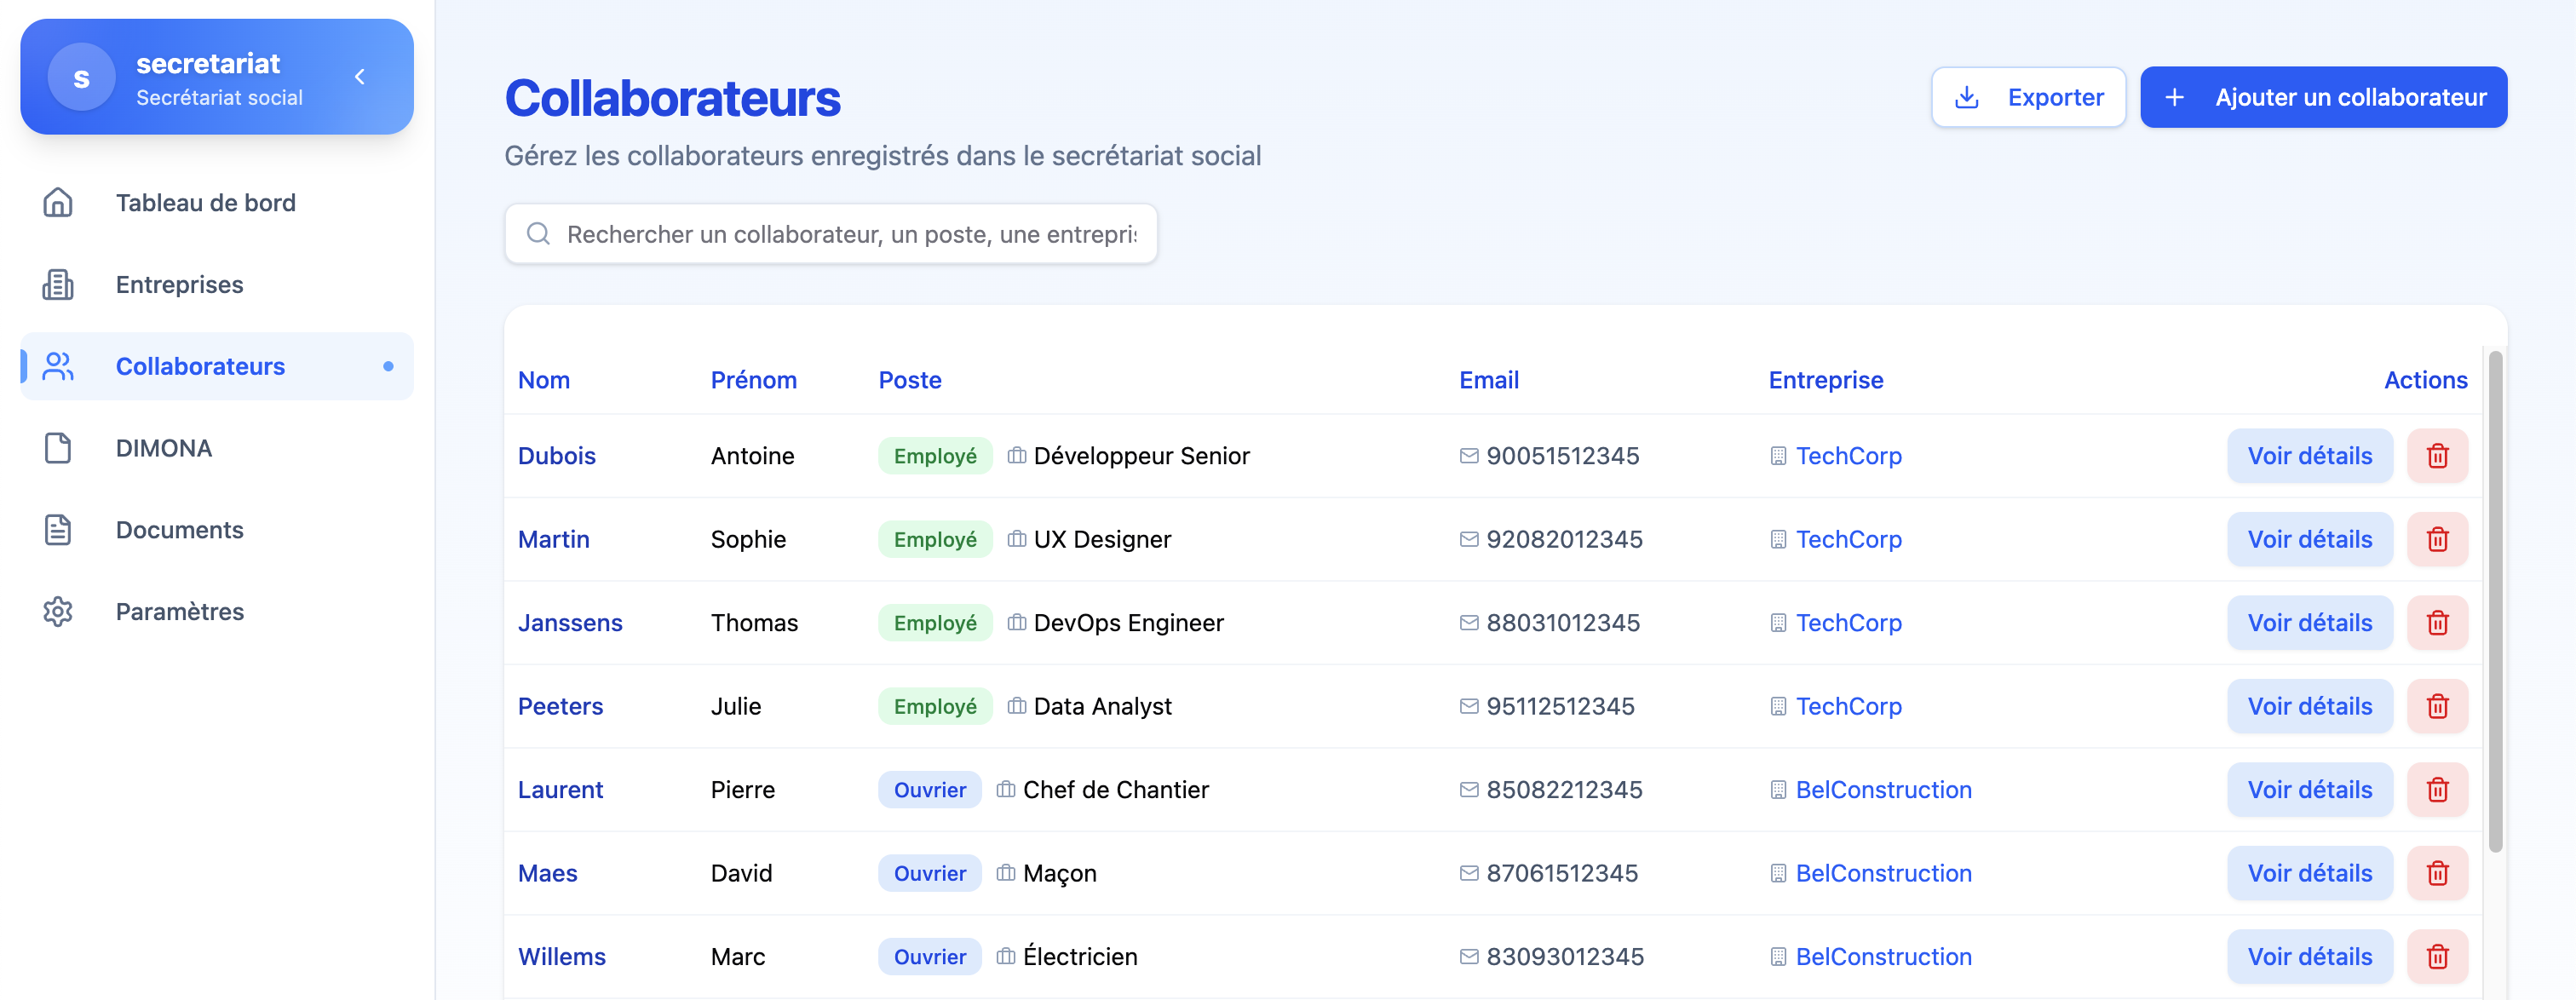
\includegraphics[width=0.9\textwidth]{SecuComPreview.png}
    \caption{Aperçu de l'interface de SecuCom}
    \label{fig:secucomPreview}
\end{figure}

\noindent Au cœur de \textbf{SecuCom} se trouve un système de gestion centralisé permettant la création, la modification et la suppression de trois types d'entités principales :
\begin{itemize}[leftmargin=*,label=\textcolor{darkgray}{$\bullet$},itemsep=0.3em]
  \item Les entreprises clientes du secrétariat social
  \item Les collaborateurs (employés) rattachés à ces entreprises
  \item Les déclarations DIMONA associées à ces collaborateurs
\end{itemize}

\vspace{0.5cm}

\noindent Contrairement aux processus manuels actuels décrits dans la section précédente, \textbf{SecuCom} offre une interface numérique unifiée qui remplace les échanges fragmentés par email et WhatsApp. Cette approche centralisée permet non seulement de réduire les risques d'erreurs lors de la saisie des données, mais aussi de faciliter le suivi et la mise à jour manuelle du statut des déclarations DIMONA, élément crucial pour la conformité légale des entreprises.

\begin{note}
L'interface utilisateur de \textbf{SecuCom} a été conçue avec une philosophie minimaliste, privilégiant la clarté et l'intuitivité. Les fonctionnalités essentielles sont mises en évidence, permettant aux utilisateurs de naviguer efficacement sans formation approfondie. Cette simplicité apparente masque cependant une architecture robuste qui gère de manière transparente les complexités des processus administratifs sous-jacents, tout en s'appuyant sur des validations internes plutôt que sur des intégrations API externes.
\end{note}

\begin{tcolorbox}[
  title={\textbf{Fonctionnalités clés de SecuCom}},
  colback=blue!5!white,
  colframe=primarycolor,
  fonttitle=\bfseries,
  boxrule=0.5mm,
  arc=2mm,
  left=6mm,
  right=6mm,
  top=6mm,
  bottom=6mm
]
\begin{itemize}[leftmargin=*,label=\textcolor{darkgray}{$\bullet$},itemsep=0.3em]
  \item La gestion sécurisée des profils d'entreprises clientes avec toutes leurs informations administratives
  \item L'encodage structuré des données des collaborateurs avec validation interne pour minimiser les erreurs
  \item La création assistée des déclarations DIMONA avec possibilité de mise à jour manuelle de leur statut
  \item Un système de notifications pour alerter les utilisateurs des actions requises ou des problèmes potentiels
  \item Une séparation stricte des accès garantissant la confidentialité des données sensibles
\end{itemize}
\end{tcolorbox}

\vspace{0.5cm}

\noindent \textbf{SecuCom} se distingue par sa \textbf{focalisation exclusive} sur les \textbf{besoins spécifiques} des secrétariats sociaux de petite taille et de leurs clients, offrant ainsi une \textbf{solution sur mesure} là où les plateformes généralistes proposent souvent des fonctionnalités superflues qui complexifient l'expérience utilisateur.

\vspace{0.5cm}

\begin{figure}[H]
  \centering
  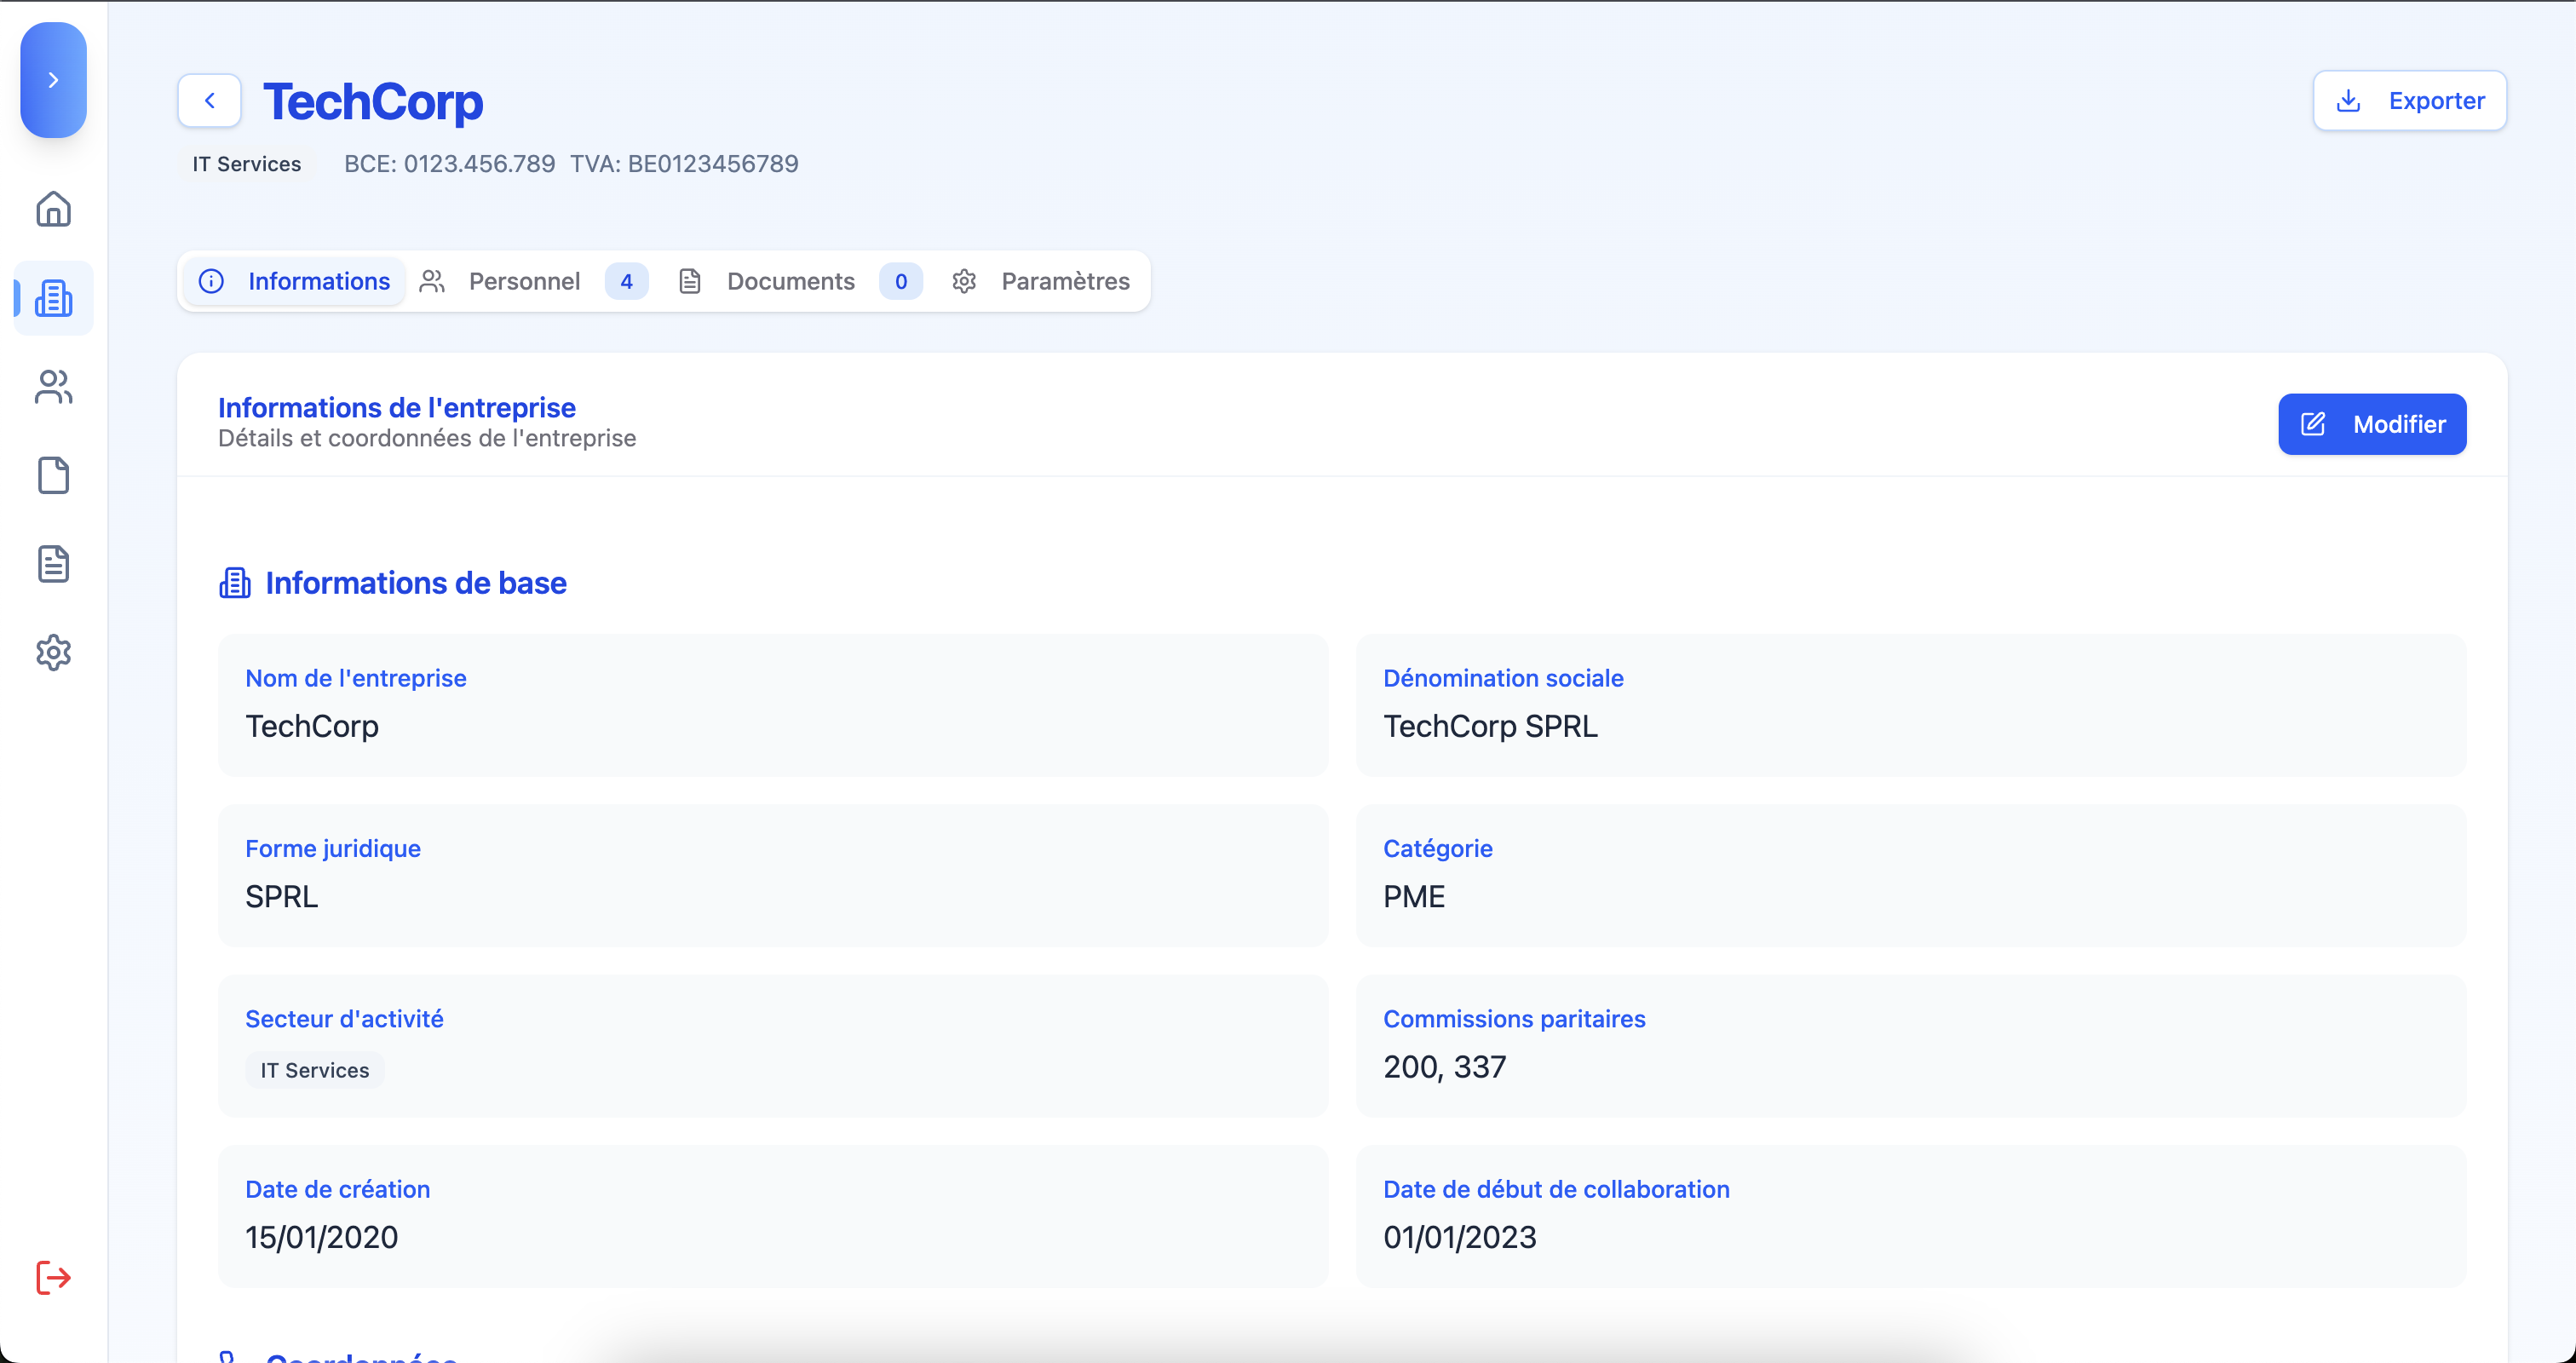
\includegraphics[width=0.9\textwidth]{SecuComPreviewCompany.png}
  \caption{Aperçu de l'interface de SecuCom}
  \label{fig:secucomPreview}
\end{figure}

\section{À qui est destiné SecuCom ?}

\textbf{SecuCom} s'adresse principalement à deux catégories d'utilisateurs, chacune avec des besoins et des niveaux d'accès spécifiques :

\subsection{Le personnel du secrétariat social (Sodabel)}

\begin{itemize}[leftmargin=*,label=\textcolor{darkgray}{$\bullet$},itemsep=0.3em]
  \item \textbf{Le personnel du secrétariat} : Les utilisateurs du secrétariat social bénéficient d'un accès complet à toutes les entreprises clientes, leurs collaborateurs et leurs déclarations DIMONA. L'interface leur permet de traiter efficacement les demandes, de vérifier les informations et d'effectuer les déclarations officielles auprès des organismes compétents.
\end{itemize}

\begin{note}
Dans la version actuelle de \textbf{SecuCom}, un seul rôle "secrétariat" est implémenté pour tous les utilisateurs de Sodabel. Une distinction plus fine entre les rôles (comme gérant et secrétaires) pourra être développée ultérieurement selon les besoins spécifiques identifiés lors de l'utilisation du système.
\end{note}

\vspace{0.5cm}

\noindent Pour ces utilisateurs, \textbf{SecuCom} offre une vue d'ensemble de tous les clients, permettant une gestion transversale et efficace des dossiers. L'interface est optimisée pour faciliter le traitement en série des demandes et la gestion simultanée de multiples entreprises clientes.

\subsection{Le personnel administratif des entreprises clientes}

\textbf{Les employés administratifs} désignés par chaque entreprise cliente ont accès à un espace privé limité aux données de leur propre organisation. Ils peuvent :
\begin{itemize}[leftmargin=*,label=\textcolor{darkgray}{$\bullet$},itemsep=0.3em]
  \item Consulter et mettre à jour les informations de leur entreprise
  \item Gérer leurs propres collaborateurs (ajout, modification, suppression)
  \item Initier des demandes de déclaration DIMONA
  \item Suivre l'état d'avancement de leurs déclarations
\end{itemize}

\vspace{0.5cm}

\noindent Pour ces utilisateurs, l'interface est simplifiée et focalisée uniquement sur leurs propres données, éliminant toute distraction ou confusion potentielle. Les actions possibles sont clairement délimitées et guidées pour minimiser les erreurs.

\begin{tcolorbox}[
  title={\textbf{Séparation des accès}},
  colback=blue!5!white,
  colframe=primarycolor,
  fonttitle=\bfseries,
  boxrule=0.5mm,
  arc=2mm,
  left=6mm,
  right=6mm,
  top=6mm,
  bottom=6mm
]
\noindent Cette séparation stricte des accès est un élément fondamental de l'architecture de \textbf{SecuCom} :
\begin{itemize}[leftmargin=*,label=\textcolor{darkgray}{$\bullet$},itemsep=0.3em]
  \item \textbf{Sodabel} peut voir l'ensemble des clients et de leurs données
  \item \textbf{Chaque entreprise} est confinée à son propre périmètre
\end{itemize}

\noindent Cette approche garantit non seulement la confidentialité des données sensibles, mais simplifie également l'expérience utilisateur en ne présentant à chacun que les informations pertinentes pour son rôle.
\end{tcolorbox}

\vspace{0.5cm}

\noindent L'interface épurée et intuitive de \textbf{SecuCom} a été spécifiquement conçue pour s'adapter à des utilisateurs ayant des niveaux variables de compétences informatiques, reconnaissant que dans de nombreuses petites entreprises, les tâches administratives sont souvent gérées par du personnel non spécialisé. Les formulaires incluent des validations intelligentes et des indications contextuelles pour guider les utilisateurs et prévenir les erreurs courantes.

\begin{note}
Les validations en temps réel des formulaires permettent de détecter immédiatement les erreurs potentielles, comme un numéro de registre national mal formaté ou une date de début de contrat incohérente, évitant ainsi des problèmes administratifs ultérieurs.
\end{note}

\vspace{0.5cm}

\begin{figure}[H]
  \centering
  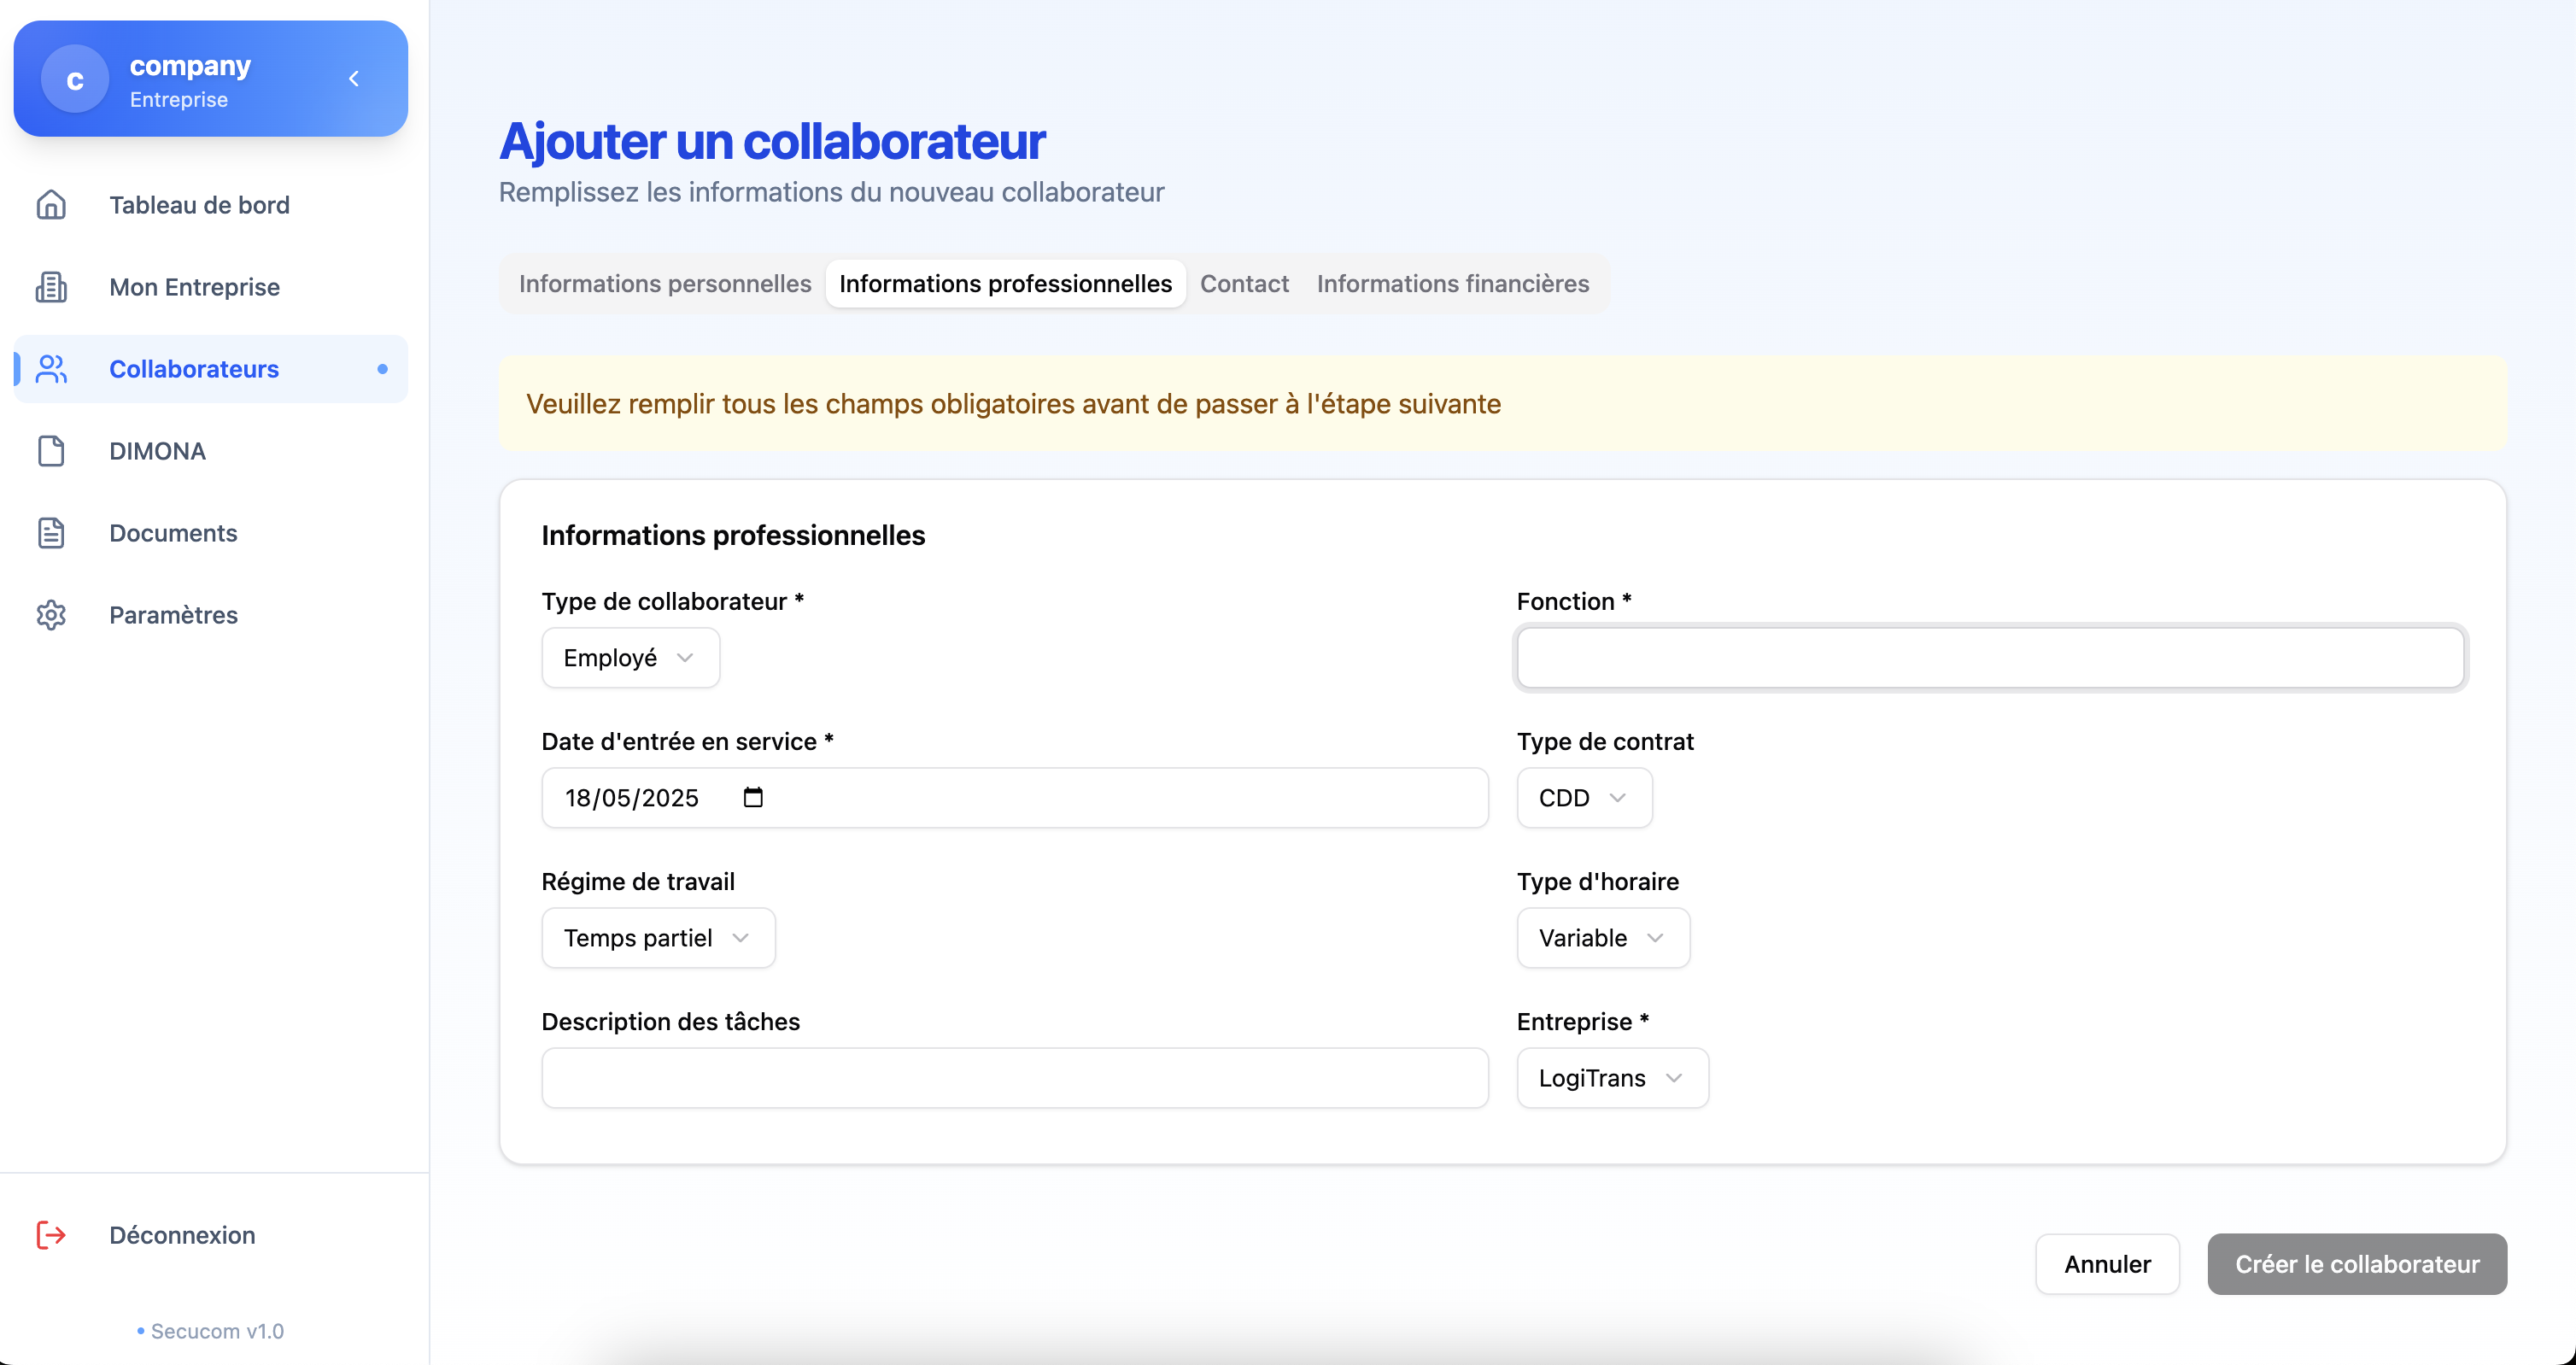
\includegraphics[width=0.9\textwidth]{SecuComPreviewCollaborator.png}
  \caption{Aperçu de l'interface de SecuCom}
  \label{fig:secucomPreview}
\end{figure}

\vspace{0.5cm}

\noindent En résumé, \textbf{SecuCom} offre une expérience sur mesure pour chaque type d'utilisateur, tout en maintenant une cohérence globale qui facilite la communication et la collaboration entre le secrétariat social et ses clients.
